\documentclass[sigconf,screen]{acmart}
% For algorithms in ACM template
\makeatletter
\newif\if@restonecol
\makeatother
\let\algorithm\relax
\let\endalgorithm\relax
\usepackage[T1]{fontenc} 
\usepackage[subtle]{savetrees}
\usepackage[ruled,vlined]{algorithm2e}
\usepackage{cleveref}
\usepackage{makecell}
\usepackage{soul}
\usepackage{tabularx}
\usepackage{enumitem}
\providecommand\algorithmname{algorithm}

\AtBeginDocument{%
  \providecommand\BibTeX{{%
    \normalfont B\kern-0.5em{\scshape i\kern-0.25em b}\kern-0.8em\TeX}}}

\begin{document}

\title{Testing Approximations for Augmented and Virtual Reality}

\author{Samuel Grayson}
\email{grayson5@illinois.edu}
\affiliation{%
  \institution{University of Illinois at Urbana-Champaign}
}

\author{Navi Ning}
\email{xning5@illinois.edu}
\affiliation{%
  \institution{University of Illinois at Urbana-Champaign}
}

\settopmatter{printacmref=false} % Removes citation information below abstract
\renewcommand\footnotetextcopyrightpermission[1]{} % removes footnote with conference information in first column

\newcommand{\todo}[1]{\textcolor{red}{#1}}

\begin{abstract}
AR/VR systems have stringent realtime performance, power, and area constraints, which are difficult to simulatenously satisfy.
One way to bring this difficulty down is through the use of \textit{approximation techniques};
    in many cases, the output only has to fool a human, so the algorithms can be simplified or reduced.
However, one does not know \textit{a priori} which approximations will `fool the human.'
This project seeks automataically determine the acceptability of approximations, so approximation-configurations can be rapidly searched.
\end{abstract}

% http://dl.acm.org/ccs.cfm
% \begin{CCSXML}
% <ccs2012>
% <concept>
% <concept_id>10011007.10010940.10010992.10010993.10010994</concept_id>
% <concept_desc>Software and its engineering~Functionality</concept_desc>
% <concept_significance>300</concept_significance>
% </concept>
% </ccs2012>
% \end{CCSXML}

% \ccsdesc[300]{Software and its engineering~Functionality}

% \keywords{approximation tuning}

\maketitle

\section{Introduction}

\begin{itemize}
\item A \ul{virtual reality} system presents the user with an opaque visual display that consumes their entire {field-of-vision}. Within this field, what the user sees is determined by estimating the \ul{pose} (position and orientation) of the users head in the real-world and {rendering} a virtual world from that pose. This gives the user the illusion of being immersed in the virtual world.

\item An \ul{augmented reality} system uses a transparent display, so virtual elements can be overlayed on the physical world. THe virtual objects should move synchronously with the physical objects they overlay, since they are rendered from the user's head-pose.

% \item A \ul{mixed reality} system uses an opaque display like virtual reality, but displays a background from the real world, emulating augmented reality.

% \item eXtended Reality (XR) system is a catch-all term for virtual reality, augmented reality, or mixed reality. \todo{cite}

\end{itemize}

There are some commercially available AR and VR systems, such as HTC Vive Pro (example of VR) and Microsoft HoloLense 2 (example of AR). However, the {quality-of-experience} in these systems can stand to be improved. In order to fully immerse the user, more resolution and a faster latency are needed. Furthermore, AR/VR systems need to be mobile/tetherless to support the full breadth of AR/VR applications, and tetherless systems imply a strict power constraint on top of the existing performance constraints. There are multiple orders of magnitude between state-of-the-art AR/VR systems and ideal futuristic systems in performance, power, and area. \todo{save space here}

%(shown in \cref{requirements}).

% \begin{table}
%   \centering
%   {
%     \caption{State-of-the-art versus ideal AR and VR performance characterstics according to \cite{huzaifa2020exploring}}
%     \scriptsize
%     \setlength{\tabcolsep}{3pt}
%     \begin{tabular}{c c c c c}
%       \textbf{Metric}       & \textbf{HTC}      & \textbf{Ideal VR} & \textbf{Microsoft}  & \textbf{Ideal AR} \\
%                             & \textbf{Vive Pro} &                   & \textbf{HoloLens 2} &                   \\ \toprule
%       Resolution (MPixels)  & 4.6 ~             & 200               & 4.4~                & 200               \\ 
%       \hline
%                             & 110~              & Full:             & 52 diagonal         & Full:             \\
%       Field-of-view         &                   & 165$\times$175    &  ~                  & 165$\times$175    \\
%       (Degrees)             &                   & Stereo:           &                     & Stereo:           \\
%                             &                   & 120$\times$135    &                     & 120$\times$135    \\ \hline
%       Refresh rate (Hz)     & 90~               & 90 -- 144         & 120~                & 90 -- 144         \\ 
%       \hline
%       Motion-to-photon      & $<$ 20~           & $<$ 20            & $<$ 9~              & $<$ 5             \\ 
%       latency (ms)          &                   &                   &                     &                   \\ \hline
%       Power (W)             & N/A               & 1 -- 2            & $>$ 7~              & 0.1 -- 0.2        \\ \hline
%       Silicon area (mm$^2$) & N/A               & 100 -- 200        & $>$ 173~            & $<$ 100           \\ 
%       \hline
%       Weight (grams)        & 470~              & 100 -- 200        & 566~                & 10s               \\ 
%       % \hline
%     \end{tabular}
%   }
%   \label{requirements}
% \end{table}

AR/VR systems typically use an IMU sensor and a pair of stereo cameras to capture the environment. The system detects visual features in the physical environment, builds up a map of them over time, and uses this map to localize itself (\ul{simultaneous localization and mapping} or \ul{SLAM}). Prior work shows that XR systems spend a significant amount of compute resources in the SLAM computation, depending on the application, platform, physical environment, and user\cite{huzaifa2020exploring}. Existing SLAM algorithms \textit{already have} approximation knobs. In fact, they have `too many;' nobody knows which ones to turn. Therefore, automatically searching for feasible SLAM approximations could greatly improve system performance.

% \section{Problem}

We wanted to build out a system \textit{in practice} not just in theory. Therefore, we built off of Illinois eXtended Reality System (ILLIXR): an open-source runtime for AR/VR applications\cite{huzaifa2020exploring}. \todo{Screenshot of ILLIXR}

This project seeks to answer or partially answer three questions:

\begin{enumerate}[label={\textbf{R.Q. {\theenumi}}}]
\item How can we test SLAM approximations in ILLIXR?
\item How can we do so \textit{automatically}?
\item How can we do so \textit{automatically} and \textit{quickly}?
  \begin{itemize}
  \item Due to time constriants, We only provide a partial implementation of this research question.
  \end{itemize}
\end{enumerate}

% ILLIXRLink{path} links to path at a fixed commit.
\newcommand{\ILLIXRlink}[1]{\href{https://github.com/ILLIXR/ILLIXR/tree/6c25003f79ecc35b4e002615b5a05d3077851d90}{\texttt{#1}}}

\section{Implementation}

\footnote{Our implementation is located at: \href{https://github.com/ILLIXR/ILLIXR/tree/illixr-testing}{\texttt{https://github.com/ILLIXR/ILLIXR/tree/illixr-testing}}}

\subsection{R.Q. 1 Approximation Testing}

With the following infrastructure, we can test out different approximations and manually inspect the output for acceptance for \textbf{R.Q. 1}.
We also need to know how much time the approximation saves, so we know if it is `worth it.'
The data we collected on compute-times are shown in \cref{compute-times}.

\begin{figure}
  \label{compute-times}
  \caption{Compute times for various approximation configurations.}
  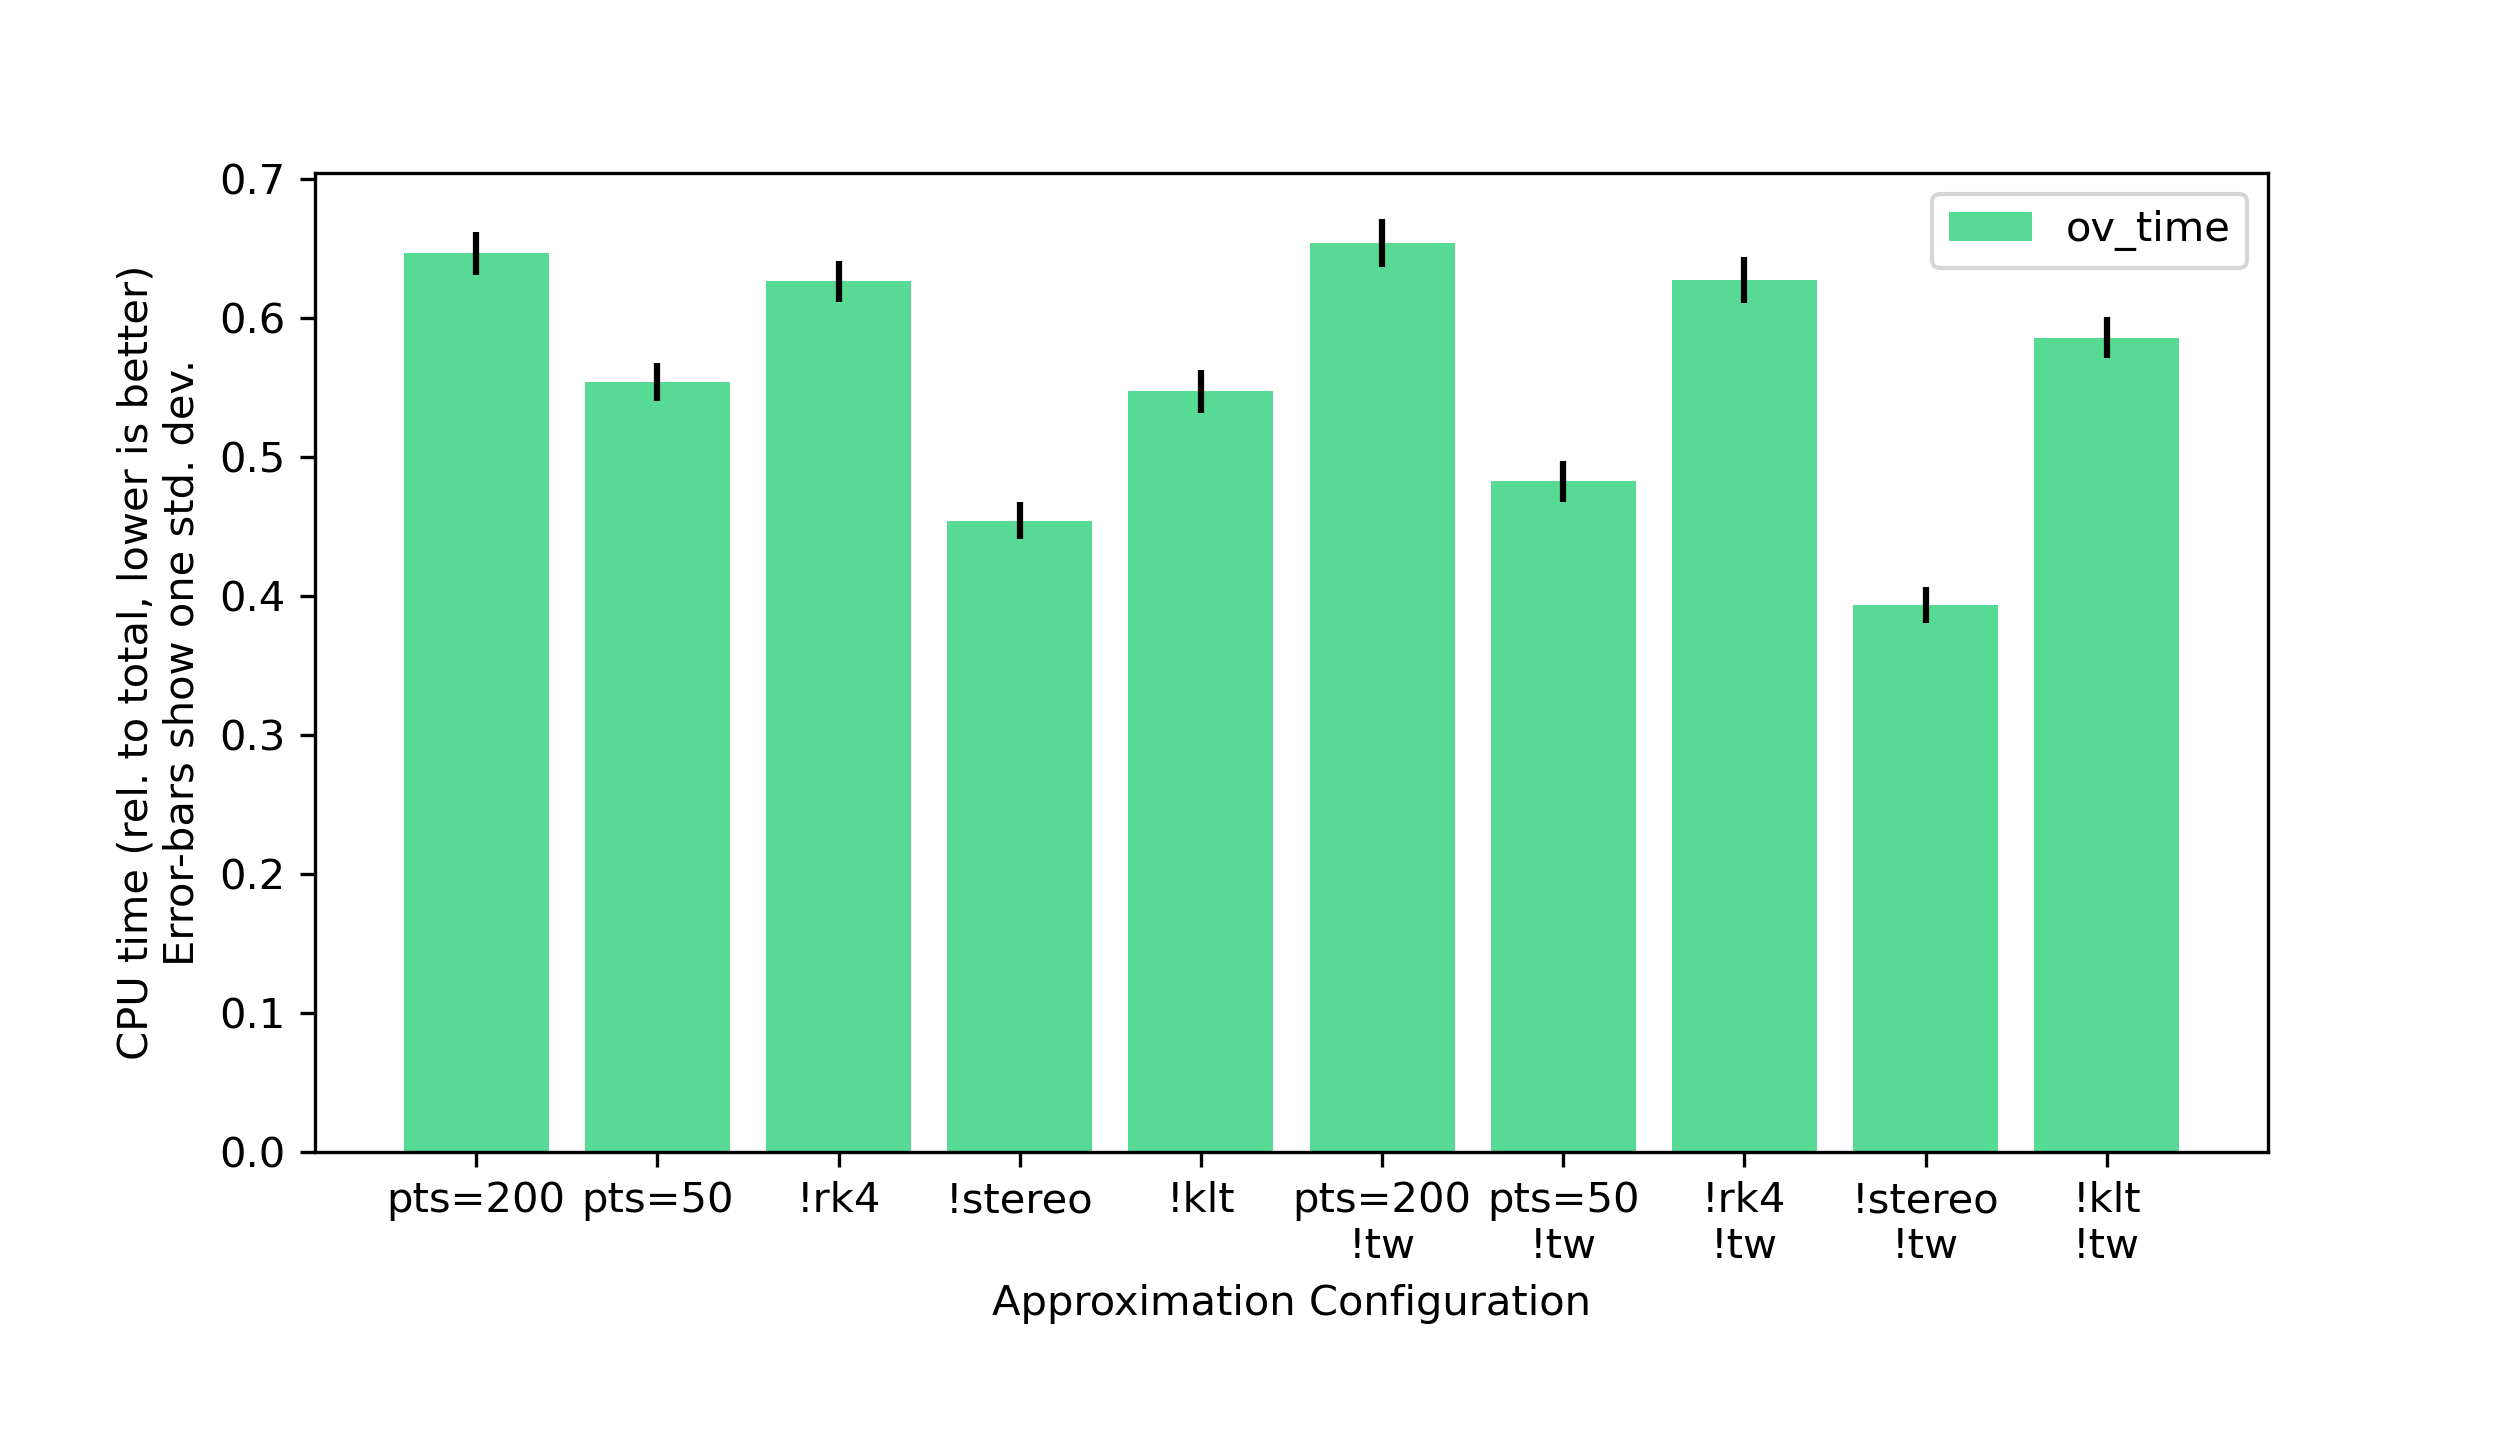
\includegraphics[width=\columnwidth]{times.png}
\end{figure}

\subsubsection{Approximation Knobs}

ILLIXR uses state-of-the-art components such as OpenVINS \cite{Geneva2020ICRA} for SLAM.
We located approximation knobs in OpenVINS and consulted domain experts on which ones should be modified and tuned.\footnote{
  \todo{href to https://github.com/ILLIXR/open\_vins/blob/illixr-testing/ov\_msckf/src/slam2.cpp\#L30}
}

\begin{table*}
  \centering
  {
    \caption{OpenVINS approximation knobs. See OpenVINS documentation for more details\cite{Geneva2020ICRA}.}
    \begin{tabularx}{\linewidth}{r||l|X}
      \textbf{Knob} & \textbf{Range} & \textbf{Meaning} \\
      & {(approx. first)} & \\
      \hline\hline
      \verb+num_pts+ & 50--300 & The number of points extracted and tracked in each image frame \\
      \verb+use_rk4_integration+ & [false, true] & If Rk4 imu integration is used\\
      \verb+use_stereo+ & [false, true] & Whether cameras are stereo or binocular. If binocular, it does monocular feature tracking on each image \\
      \verb+use_klt+ & [false, true] & Uses KLT tracking or descriptor matcher \\
      \verb+downsample_camera+ & [true, false] & Halves the resolution all tracking image \\
      \verb+enable_async_reproject+ & [false, true] & (outside of OpenVINS, elsewhere in ILLIXR) queries a current pose and reprojects the frame just before display, making up for some latency in SLAM \\
    \end{tabularx}
  }
\end{table*}

The exact set of knobs is not so significant, as long as I have some useful ones, some useless ones, and they are orthogonal.

\subsubsection{Timing Infrastructure}

In order to test the approximations, I need to know how much time they are saving. Timing ILLIXR is not straightforward.
\begin{itemize}
\item Whole-program CPU time won't work because, because ILLIXR will find another way to spend the spare cycles.
\item \verb+perf+ won't work because it does not have dynamic information (the arguments) of the function. It is thus impossible to disambiguate which component to charge a function-call to.
\item Language-level tools won't work because they are oblivious to threads launched and joined inside a function. Several functions in OpenVINS launch a short-running thread to parallelize the computation.
\end{itemize}

Since none of these off-the-shelf solutions will work, we created a lightweight framework for CPU time logging.
At each function one wants to instrument, one can call a macro with a static label (such as a function name) and dynamic label (such as arguments that disambiguate the function-call).
We use \verb+clock_gettime+ to measure the actual time the thread spends scheduled.
We use resource-acquisition-in-initialization RAII to automatically time the enclosing scope.
Creating the RAII object pushes the current call onto a thread-local stack.
These stack-frame times get pushed onto a global list and serialized only at the very end of the program, so as to not perturb performance during execution\footnote{\todo{href to common/cpu\_timer3.hpp}}.

\subsection{R.Q. 2 Automatic Approximation Testing}

In order to automatically accept or reject approximations, we collect system-level error metrics.
In a real system, we would determine a threshold of acceptability from user-studies, but that is outside the scope of this project;
    we will continue under the assumption that \textit{there is some} threshold.

The data we collect is shown in \cref{system-level-errors}.
Unfortunately, there seems to be a large variance in the system-level errors across frames (their standard deviation is larger than their mean and median).
This means some frames look basically the same, and some have huge differences.
Future work could investigate why this is.
Defining a video metric for AR/VR is still an open problem, and our \textbf{R.Q. 2} system enables research into that question.

\begin{figure}
  \label{system-level-errors}
  \caption{System-level error for various approximation configurations.}
  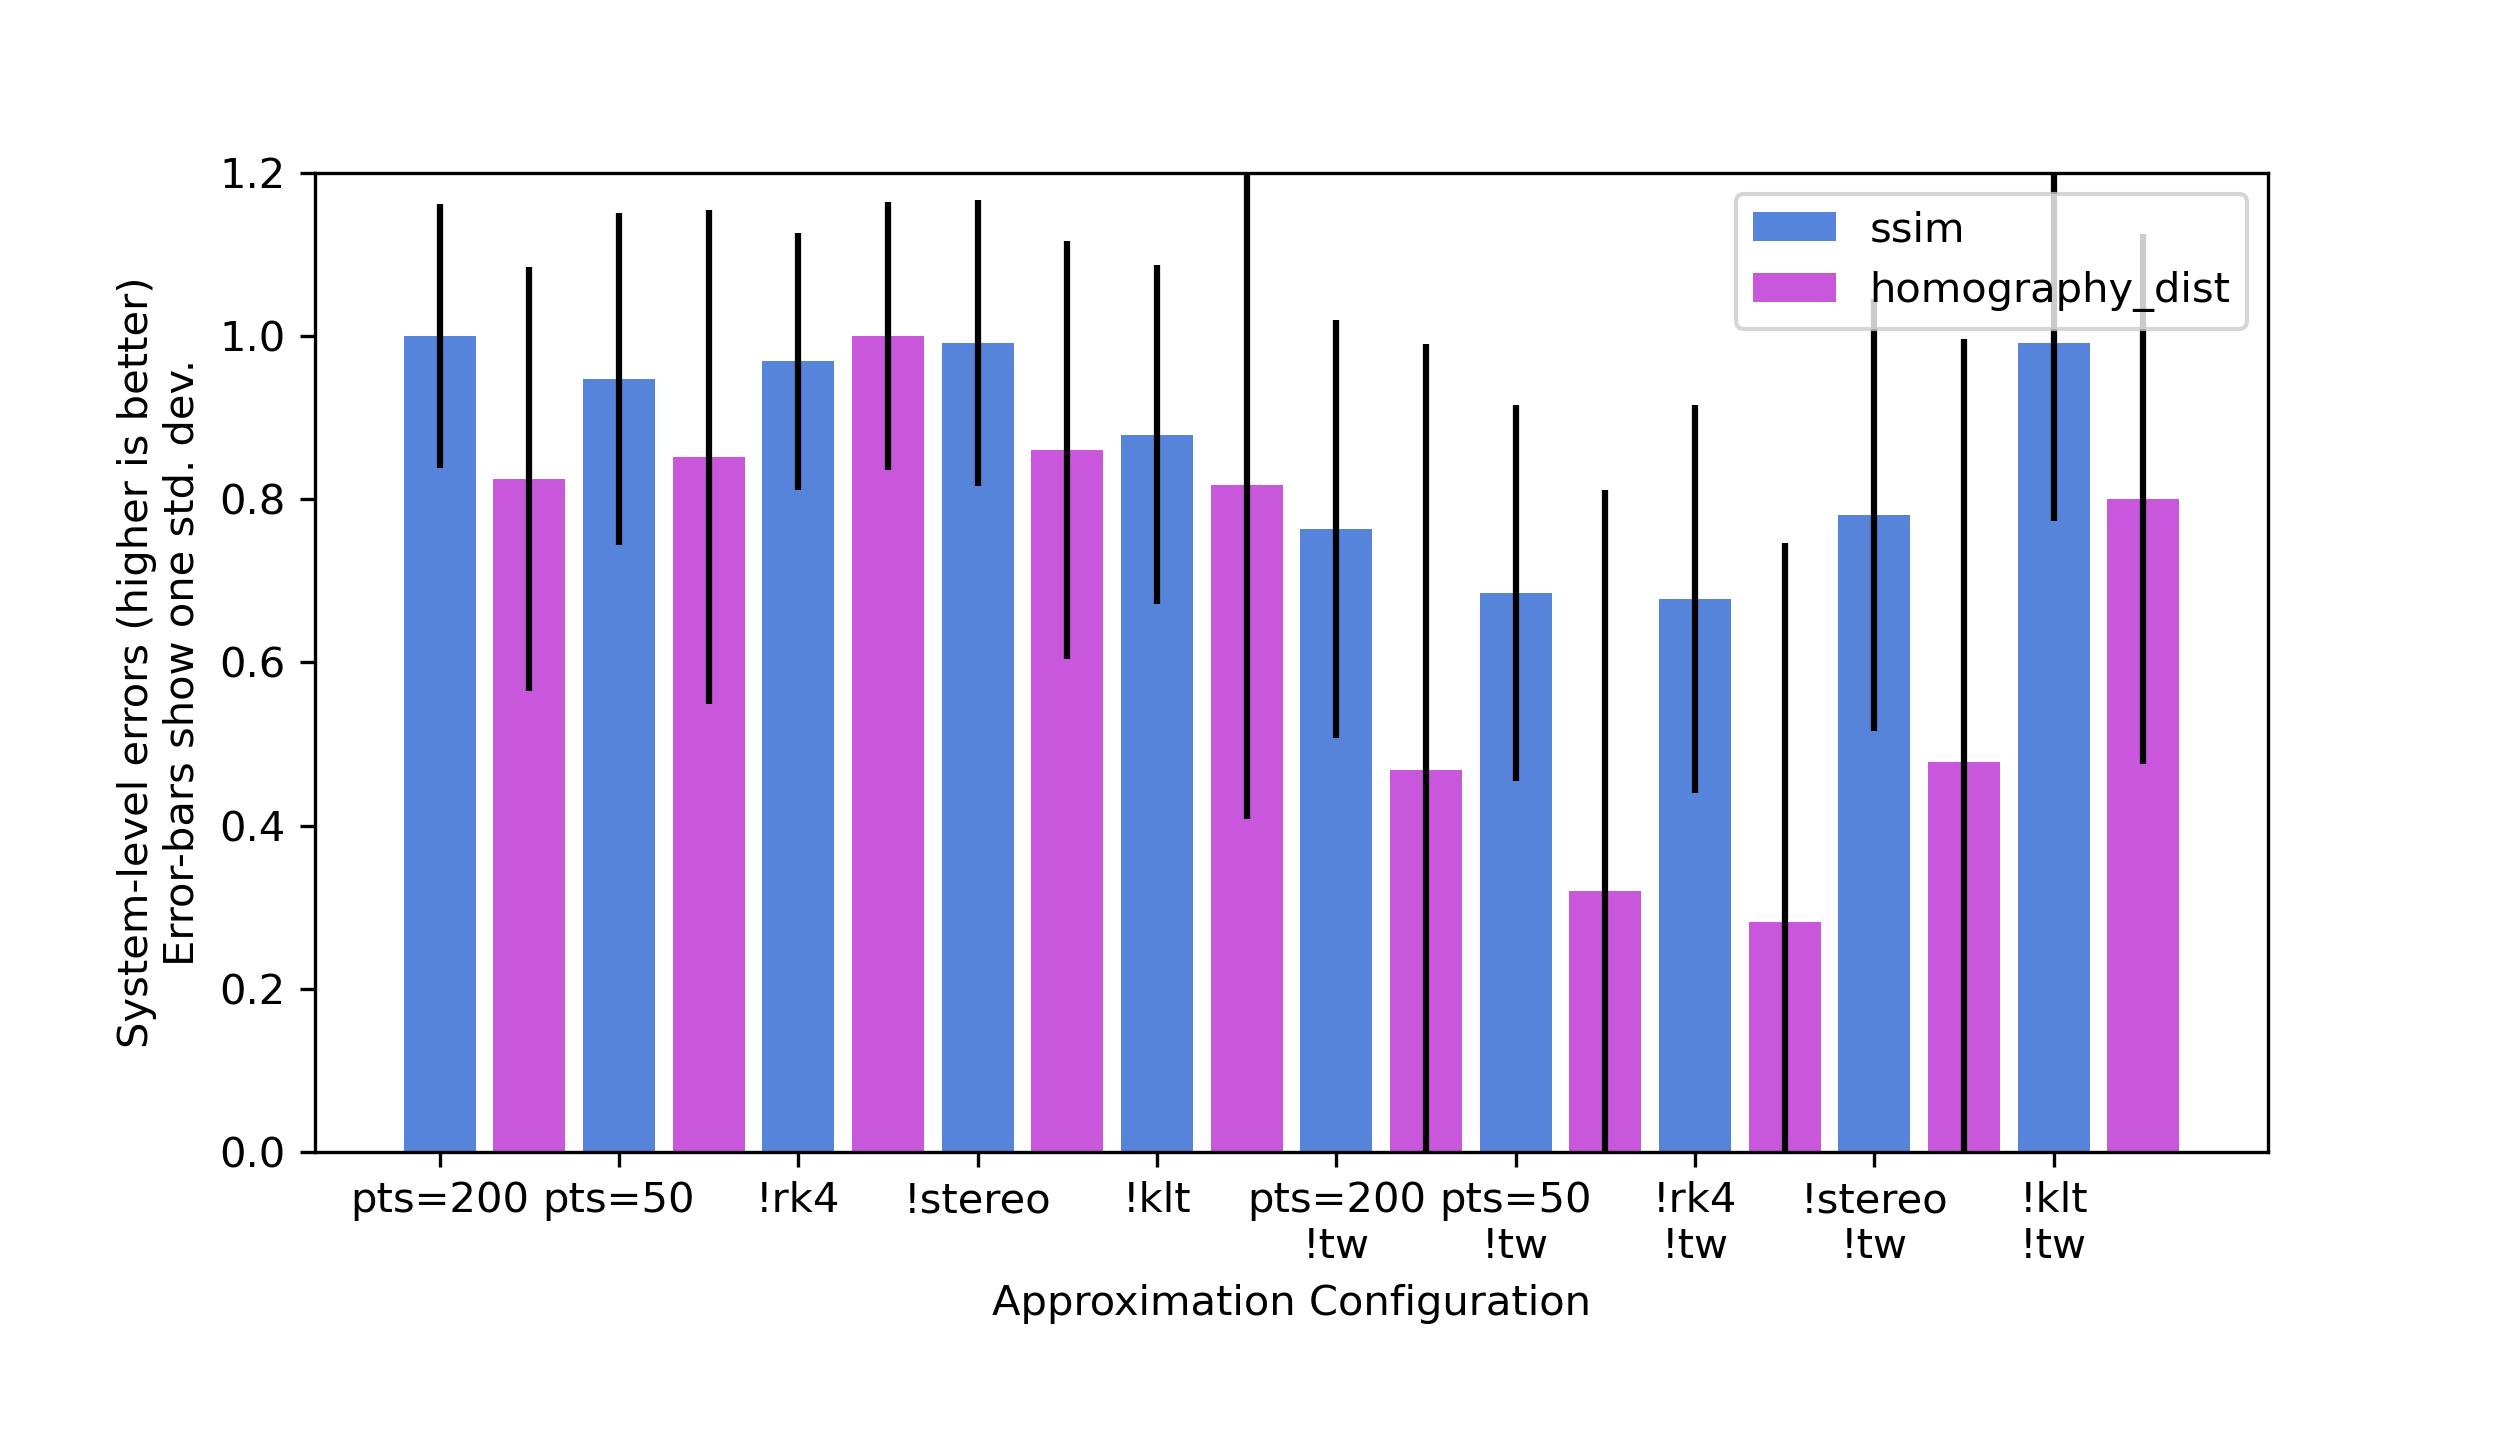
\includegraphics[width=\columnwidth]{system_errors.png}
\end{figure}

\subsubsection{Approximation Configuration Infrastructure}

We created a script that runs ILLIXR over an arbitrary set of approximation configurations.
The script configures ILLIXR by generating an ILLIXR configuration file and environment variables.\footnote{\todo{href to experiment.py:run\_illixr}}

\subsubsection{System-Level Metrics}

In the interest of repeatability, we switched to ILLIXR's offline-mode which uses a dataset on disk instead live sensor data.
We used the EuRoC dataset, which has high-quality ground-truth pose data \cite{Burri25012016}.

The output of an XR system with pre-recorded sensor trace is essentially a video stream.
Capturing the video-stream is non-trivial because dumping frames eagerly would perturb the computation, while deferring until the end of the computation involves buffering which has proven too memory intensive.
Since ILLIXR uses OpenGL commands to draw frames, we can just capture every OpenGL command in a binary format and replay those commands offline.
This is exactly what the \verb+apitrace+ tool does \cite{apitrace}.\footnote{\todo{href to experiment.py:159}}

We generate that video-stream from the ground-truth data, and then compare the two frame-by-frame.
First, we tried using Structural Similarity Index Metric (SSIM), which has been used to compare XR video streams before \todo{citation}\footnote{\todo{href video\_dist.py:compute\_ssim}}.
However, this may not be the best metric to compare video streams which have variation in their pose.

With SSIM performing poorly, we also tried a hand-made metric we call \ul{homography-distance}:
For each frame of the both videos, we use SIFT to identify comon features in both frames \todo{cite SIFT} and take the mean difference in position (we also tried median and max difference).\footnote{\todo{link to video\_dist.py:compute\_feature\_dist}}
Like a user, it emphasizes rotations (in which every pixel moves) over translations (in which only pixels on foreground objects move).
Most of the inaccuracies in homography-distance correspond to valid relaxations of user acceptance.
For example, SIFT will be unable to detect many features if the background is uniform (say your looking at a blue sky),
    but a human user, unable to lock onto any feature, would also be less able to detect small movements and would be more forgiving.

\subsection{R.Q. 3 Fast Automatic Approx Testing}

The prior method involves running the whole system for one minute (enough time to collect a representative trace), about two minutes to replay the OpenGL trace, and ten minutes to compute the video distances.
Ideally, we could use approximation auto-tuning such as ApproxHPVM \cite{approxhpvm}, but this goal is still quite far away. First, we need to evaluate system-level effects of approximations at a much faster rate.

\subsubsection{Estimating System-Level Error by Component-Level Proxies}

The component-level metrics are much easier to get than the system-level ones.
Only a small set of components have to be run, and they can be run without realtime scheduling (no need to \verb+sleep+ to get the timing right).
Determining the system-level error from the component-level error analytically is too difficult.
AR/VR systems have multiple paths from SLAM to the output, which makes the error \textit{non-compositional}.
For example, errors SLAM at time \(t\) in render can be corrected by SLAM at \(t+\delta\) through the timewarp (in \cref{dag}).

\begin{figure}
\caption{AR/VR DAG, showing how SLAM flows to the output over multiple paths.}
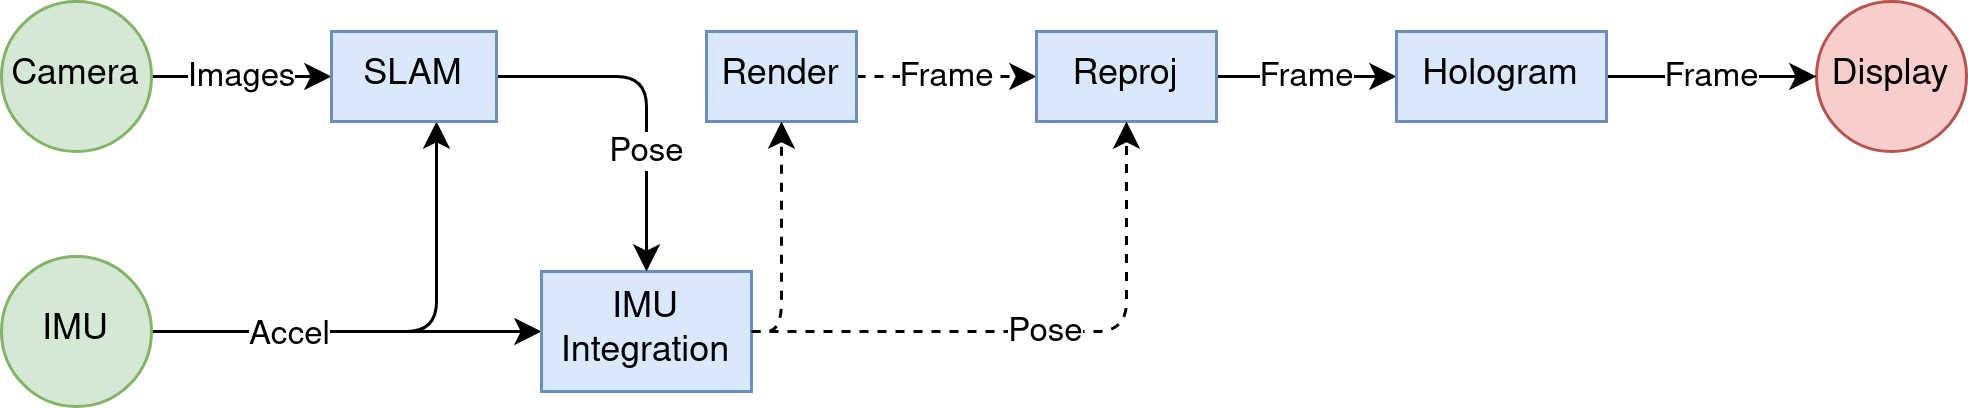
\includegraphics[width=\columnwidth]{dag.png}
\label{dag}
\end{figure}

Instead of an analytical model, we might consider an empirical one, using machine learning techniques.
It is possible that the effect of different component-level errors is non-compositional;
Therefore, a two- or three-layer fully-connected neural network will probably be able to capture the mapping from component-level error to system-level error.

\subsubsection{Component-Level Metrics}

For SLAM-level metrics, we compare the poses SLAM returned to the ground-truth.
However, since the ground-truth data was collected by different sensors, it is stored in a different frame-of-reference.
We used the Umeyama's Method to register a correspondence from SLAM's poses to the ground-truth dataset for one for a non-approximate SLAM\cite{88573}.
This provided the coordinate transformation we could use for the rest of the approximation-trials.\footnote{This alignment applies to the System-Level video metrics as well; \todo{href to ILLIXR/common/pose\_prediction:gt\_transform}}
This transformation is shown in \cref{transformation}.

\begin{figure}
  \label{transformation}
  \caption{Unaligned and aligned poses, with dotted arrows showing the transformation}
  \footnote{It only appears that the transformation `distorts' space because the transformation rotates `out of the plane'. This is a 2d projection of a 3d trajectory, so there is a part of the trajectory you can't see.}
  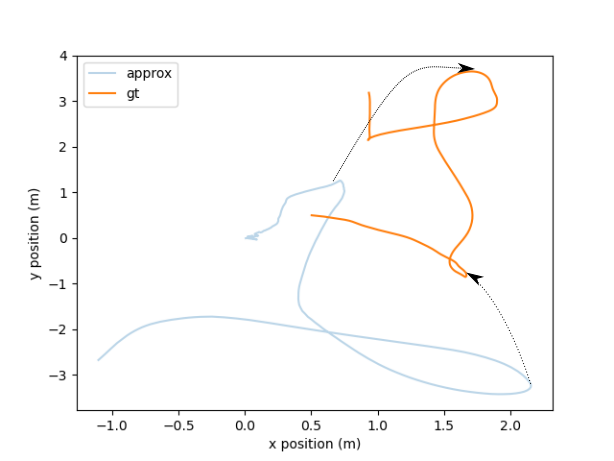
\includegraphics[width=\columnwidth]{unaligned.png}
  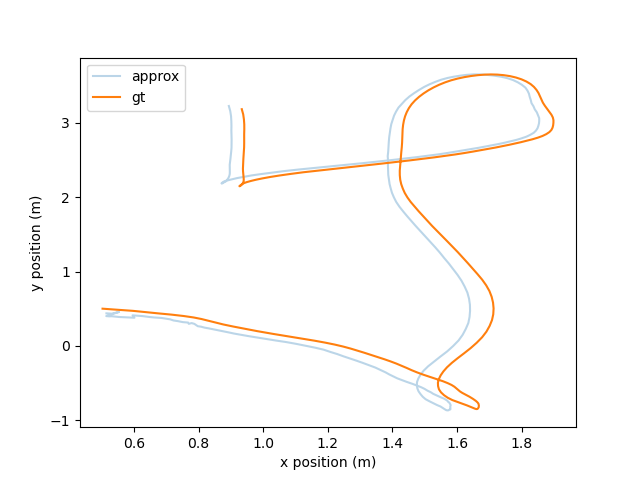
\includegraphics[width=\columnwidth]{aligned.png}
\end{figure}

We compute the euclidean distance in position-displacement the angular distance of the orientation-displacement.
These errors have a vastly different impact on users.
Rotations are the most important movement, because even if the user only moves a few degrees, everything in the world moves by an appreciable pixel-distance;
However, with translation, distant objects stay in roughly the same place. Only foreground items respond to head-translations.
Notice that mean-homography-distance implicitly captures this too:
if every object in the scene moves roughly the same amount due to rotation and a few objects in the foreground move due to translation, then the mean distance will be mostly influenced by the background but a little by the foreground too.
The component-level error we collected is also shown in \cref{SLAM-level-errors}.

\begin{figure}
  \label{SLAM-level-errors}
  \caption{SLAM-level error for various approximation configurations.}
  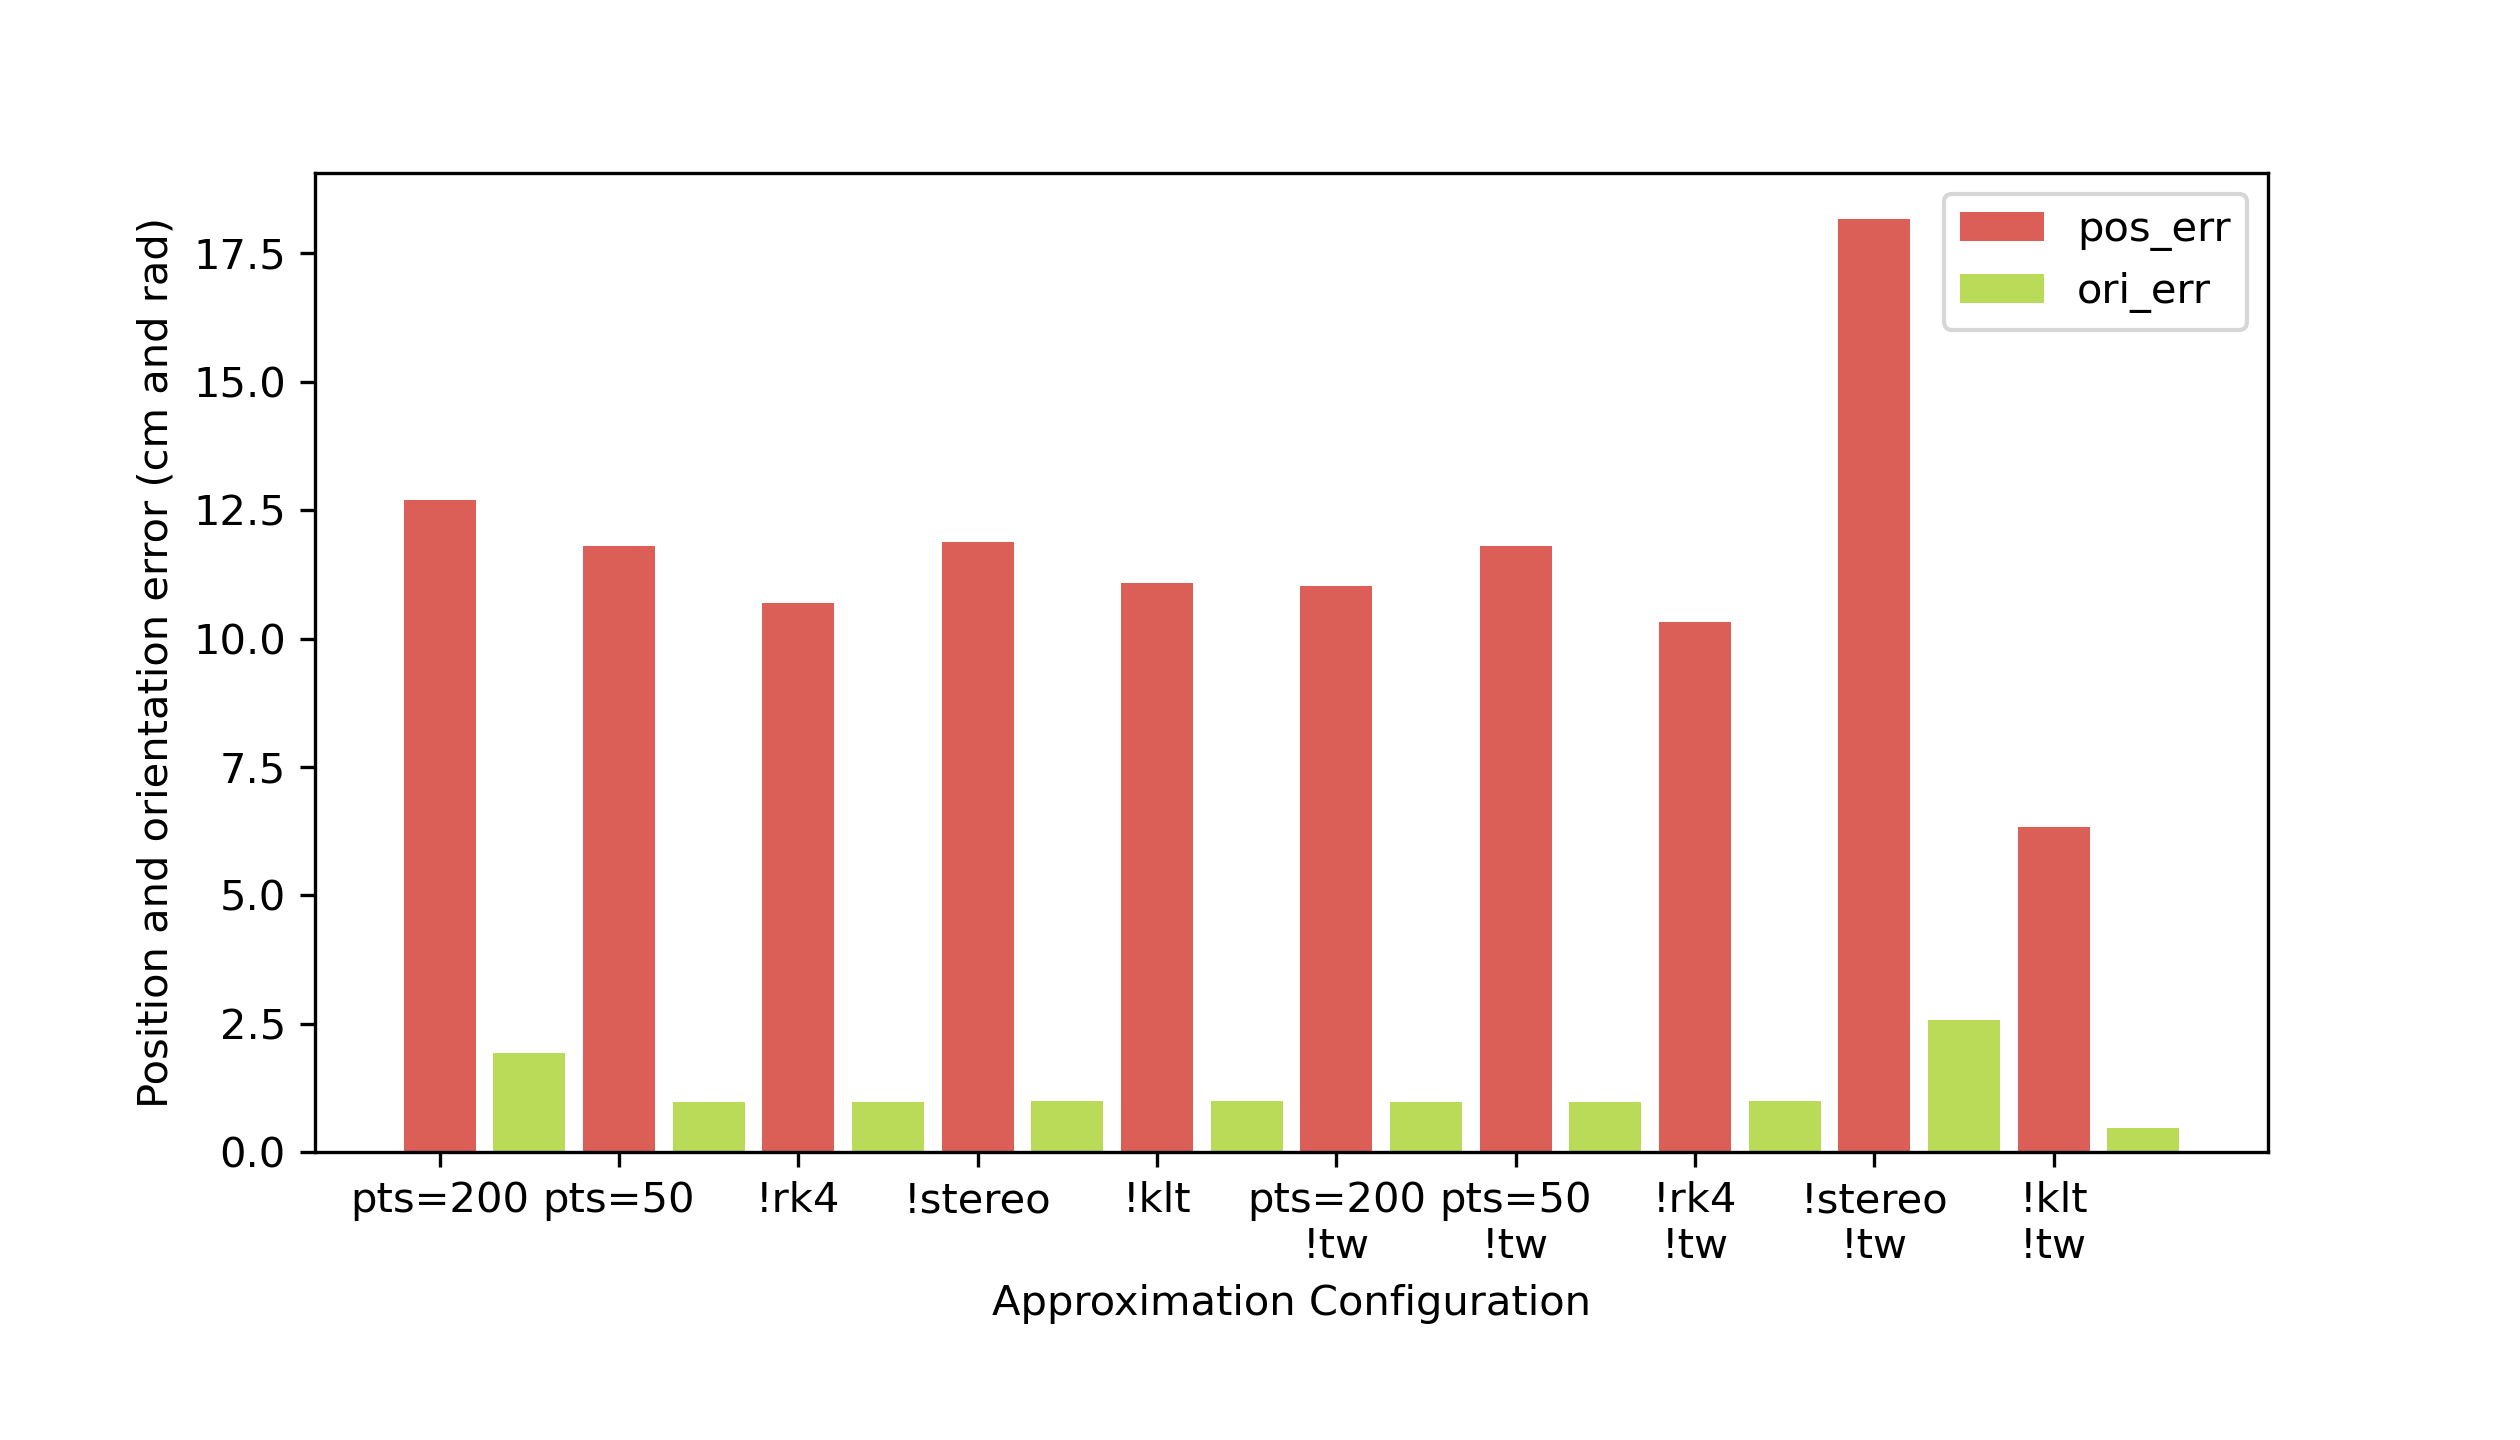
\includegraphics[width=\columnwidth]{slam_errors.png}
\end{figure}

\section{Discussion}

Many of the challenges were due to nitty-gritty engineering details. For example, actually getting the transformation right took a lot of time and debugging. Using thread-local and global variables for the CPU timers was also especially challenging. There were a few bugs that we had to work-around rather than fix, such as a race condition in the graphics code. This is the regular pain of working on a large research project.

This also implies that many of the improvements we made were engineering details that we can upstream. Trying to actually use ILLIXR to do a course project has given myself (Sam speaking) more ideas for improving it than when I was thinking about improving it full-time!

\section{Conclusion}

In just one semester, we designed and implemented a system that answers \textbf{R.Q. 1} and \textbf{R.Q. 2}. We have set groundwork for \textbf{R.Q. 3}. We also propose and evaluate a novel video distance metric. Along the way, we made software-engineering improvements on ILLIXR will be incorporated into the mainline in the near future.


% \begin{acks}
% We would like to acknowledge the ILLIXR group at the University of Illinois at Urbana-Champaign for the ILLIXR research platform itself and timely support. Specifically, we would like to thank Boyuan Tian and Yihan Pang for helping with the trajectory alignment and Muhammed Huzaifa for the coordinate transformation.
% \end{acks}

%%
%% The next two lines define the bibliography style to be used, and
%% the bibliography file.
\bibliographystyle{ACM-Reference-Format}
\bibliography{main}

\appendix
\section{Pre-existing and Concurrent Work}
This work was \textit{not} done for this project:

\begin{itemize}
\item OpenVINS already had tunable parameters.
\item ILLIXR already had timing infrastructure, but it was insufficient for our purposes, because it could not be adapted to time \textit{inside} OpenVINS.
\item The ILLIXR research group had already considered using SSIM, but their implementation was not ready at the time we needed one, so we implemented it ourselves. We could not upstream our implementation because theirs is able to handle a wider class of applications.
\item The ILLIXR research group helped me find and use Umayama's Method for aligning the pose.
\end{itemize}

This work was for this project:

\begin{itemize}
\item We designed and implemented a the infrastructure for configuring approximations across all of ILLIXR (not just OpenVINS).
\item We rewrote the timing infrastructure (from scratch).
\item We implemented component-level metrics.
\item We implemented the coordinate transformation code.
\item We implemented our own version of system-level metric (apitrace, SSIM, homography-distance).
\item We designed and implemented our own video metric (homography-distance).
\item We explored the idea of a estimating system-error by component-level proxy specifically for this projet.
\end{itemize}

\section{Total Effort}

We spent about 150 hours on this project collectively.

See our changes in ILLIXR:
\url{https://github.com/ILLIXR/ILLIXR/compare/illixr-testing?expand=1}.

See our changes in OpenVINS:
\url{https://github.com/ILLIXR/open\_vins/compare/realsense...ILLIXR:illixr-testing?expand=1}.

Note that the first few commits in our OpenVINS branch are not ours, since we merged with upsteram.

\section{Progress 6 Report}

Since progress report 5, we:

\begin{itemize}
\item designed and implemented a homography-distance.
\item designed and implemented timing infrastructure.
\item analyzed and visualized the data collected from our experiments (timing, component-level distance).
\end{itemize}

\end{document}
\endinput
